\section{ХОД РАБОТЫ}

\subsection{Постановка задачи}

Лабораторная работа состоит из двух частей. В первой части необходимо написать
программу на языке C, которая будет строить график зависимости температуры,
выраженной в градусах Цельсия и градусах Фаренгейта. Конвертацию температуры
должна осуществлять процедура, написанная на ассемблере.

Во второй части лабораторной работы требуется организовать вызов процедуры
языка высокого уровня из ассемблера (на примере вычисления факториала).

\subsection{Вызов процедура ассемблера из языка C}

Напишем модуль на языке C, который будет вызывать внешнюю процедуру, написанную
на ассемблере. Данная процедура будет конвертировать градусы по шкале Цельсия в
градусы по шкале Фаренгейта. Вызов процедуры из языка С будем вызывать в цикле,
таким образом сможем получить результаты для нескольких значений. Используя
полученные данные, построим диаграмму зависимости темперутурных шкал.

Прототип вызываемой из языка C ассемблерной процедуры с модификатором
\textit{extern} представлен на рисунке~\ref{lst:prototype}.
\begin{lstlisting}[caption=Прототип функции CF,
label=lst:prototype,language={C},basicstyle=\scriptsize\ttfamily]
 ...
 extern "C" void CF(char *buff, int *val_len, int *dot_pos, int *sign_val);
 ...
\end{lstlisting}

Рассмотрим передаваемые аргументы подробнее:

\begin{itemize}

  \item buff --- вычисляемое значение, хранимое в формате указателя на массив из цифр;
  \item val\_len --- длина массива buff;
  \item dot\_pos --- позиция разделителя (запятой);
  \item sign\_val --- знак передаваемого числа.

\end{itemize}

Все аргументы процедуры CF передаются по указателю для того, чтобы была возможность
изменять их в модуле на языке Ассемблер напрямую.

\newpage
Описание процедуры CF на языке Ассемблер приведено на рисунке~\ref{lst:proc}.
\begin{lstlisting}[caption=Описание процедуры на языке Ассемблер,
label=lst:proc,language={[x86masm]Assembler},basicstyle=\scriptsize\ttfamily]
 public _CF
 _CF proc far
     push bp
     mov  bp, sp
     push es
     push ds
     push si

     ...

     pop si
     pop ds
     pop es
     pop bp
     ret
 _CF endp
\end{lstlisting}

Учитывая тот факт, что процедура описана с модификатором far означает, что для
доступа к первому аргументу необходимо сделать смещение относительно базы на
шесть байт: bp + 6. Но стоит учесть, что аргумент процедуры --- дальний указатель,
который занимает четыре байта. Он состоит из адреса сегмента данных и адреса смещения.
Для получения значения по дальнему указателю необходимо проделать операции,
приведенные на рисунке~\ref{lst:ptr2local}.

\begin{lstlisting}[label=lst:ptr2local,caption={Запись значения, получаемого
по дальнему указателю в локальную память},language={[x86masm]Assembler},basicstyle=\scriptsize\ttfamily]
 ...
 ; construct far_ptr value
 mov ds, word ptr [ far_ptr_src + 2 ]
 mov si, word ptr [ far_ptr_src ]
 mov ax, [ds:si]

 ; set local data segment
 mov bx, @data
 mov ds, bx

 ; write data pointed by far_ptr to local mem
 mov mem_dest, ax
 ...
\end{lstlisting}

Для того чтобы исключить проблему дублирования кода, а также упростить читаемость
кода процедуры CF, создадим макрос, который будет записывать значения по дальнему
указателю в локальную память ассемблерного модуля.

Шаблон описания такого макроса приведен на рисунке~\ref{lst:macro}.
\begin{lstlisting}[label=lst:macro,caption={Шаблон описания макроса, используемого
  для записи значения в локальную память по дальнему указателю},
  language={[x86masm]Assembler},basicstyle=\scriptsize\ttfamily]
 ...
 ; copy value pointed by far ptr to local memory
 ptr2local_word macro far_ptr_src, mem_dest
   push ds
   push si
   ...
   pop si
   pop ds
 endm
 ...
\end{lstlisting}

Написанные макросы позволят упростить читаемость фрагментов кода процедуры
для изъятия аргументов из стека и записи их в локальную память:

\textit{ptr2local\_word bp+10, len\_a}

Данная команда запишет значение, хранимое в стеке по адресу bp+10 в локальную
память len\_a. Аналогичным образом создадим макросы для выполнения обратной
процедуры --- перезаписи значений, хранимых по указателю в стеке в соответствии
со значениями, хранимыми в локальной памяти.

Результат работы программы приведен на рисунке~\ref{pic:part_1}.

\begin{figure}[h!]
  \centering
  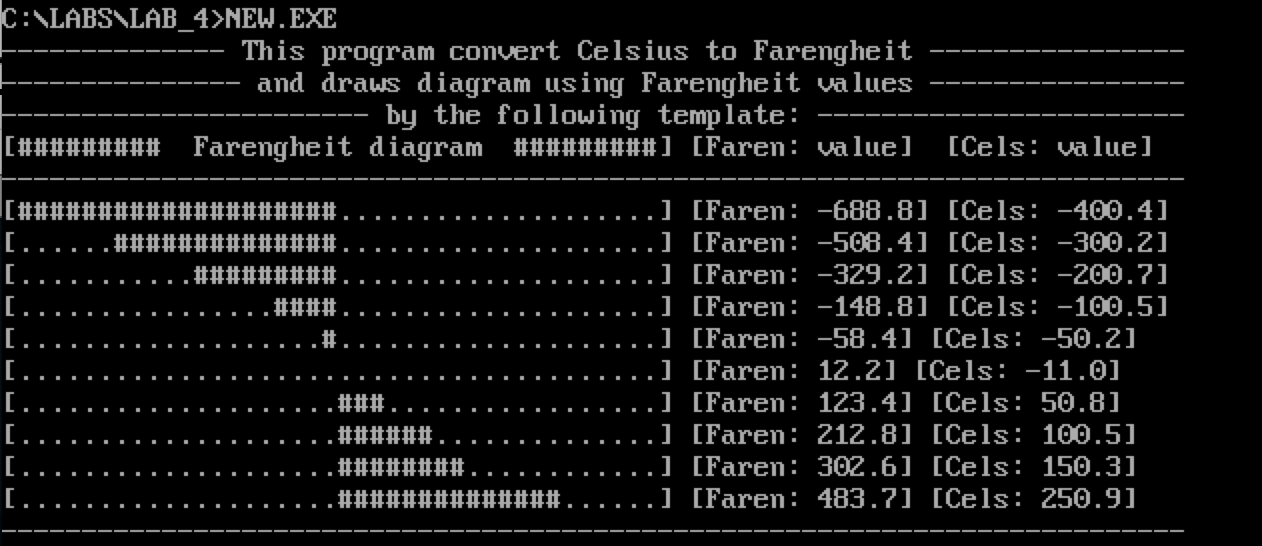
\includegraphics[width=0.8\linewidth]{pic/part_1}
  \caption{Результат работы программы построения диаграммы температурной зависимости}
  \label{pic:part_1}
\end{figure}

Исходный текст разработанной программы находится в приложении~А.

\subsection{Вызов процедур и функций языка C из ассемблера}

Разработаем в соответствии с заданием программу на языке Ассемблер, 
которая использует объектный модуль, написанный на языке C.
Разработка будет производиться под управлением 64-битной операционной системой 
на базе ядра linux (arch linux).

Объектный модуль, написанный на языке С, приведен на рисунке~\ref{lst:factorial_c}.

\begin{lstlisting}[caption=Исходный текст модуля на языке C,
label=lst:factorial_c,language={C},basicstyle=\scriptsize\ttfamily]
 unsigned long
 factorial(unsigned long x) {
   if (x == 0)
     return 1;
   else
     return x * factorial(x-1);
 }
 
 void
 flush_stdin() {
   while (getchar() != '\n');
 }
\end{lstlisting}

В данном модуле находятся две функции:
\begin{itemize}
\item factorial --- производит вычисление факториала своего аргумента рекурсивным методом;
\item flush\_stdin --- вспомогательная функция, выполняющая очисткку потока ввода.
\end{itemize}

Эти функции вызываются в основном модуле программы, написанном на языке Ассемблер, 
как показано на рисунке~\ref{lst:factorial_call_asm}.

\begin{lstlisting}[caption=Вызов процедуры вычисления факториала,
label=lst:factorial_call_asm,language={[x86masm]Assembler},basicstyle=\scriptsize\ttfamily]
 global main
     
 extern factorial

 ...
 mov     rdi, [input]
 call    factorial
 mov     [result], rax
 ...
\end{lstlisting}

Здесь четко видно, что передача параметров вызываемой процедуре осуществляется через 64-битный
регистр rdi, а возвращаемое значение --- через rax.

Результат работы программы приведен на рисунке~\ref{pic:part_2}.

\begin{figure}[h!]
  \centering
  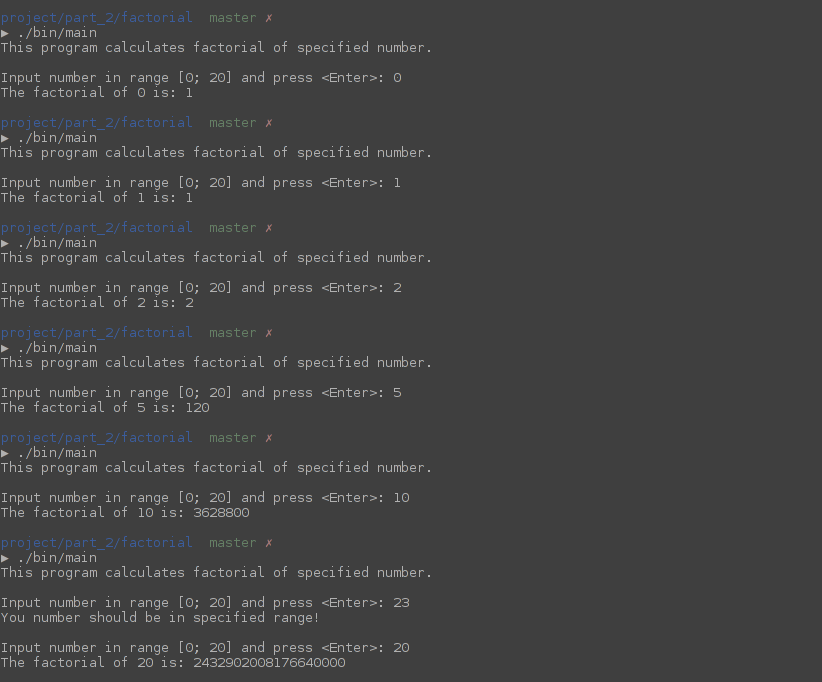
\includegraphics[width=0.8\linewidth]{pic/part_2}
  \caption{Результат работы программы \\ вычисления факториала}
  \label{pic:part_2}
\end{figure}

Исходный текст разработанной программы находится в приложении~Б.
